\documentclass[12pt,utf8,notheorems,compress,t]{beamer}
\usepackage{etex}

\usepackage[ngerman]{babel}

\usepackage{mathtools}
\usepackage{booktabs}
\usepackage{array}
\usepackage{ragged2e}
\usepackage{multicol}
\usepackage{tabto}
\usepackage{xstring}
\usepackage{soul}\setul{0.3ex}{}
\usepackage[all]{xy}
\xyoption{rotate}
\usepackage{tikz}
\usetikzlibrary{calc,shapes.callouts,shapes.arrows,patterns}
\hypersetup{colorlinks=true}

\usepackage[protrusion=true,expansion=true]{microtype}

\setlength\parskip{\medskipamount}
\setlength\parindent{0pt}

\title{Anwendungen der internen Sprache von Topoi in der algebraischen
Geometrie}
\author{Ingo Blechschmidt}
\date{October 16th, 2017}

\useinnertheme[shadow=true]{rounded}
\useoutertheme{split}
\usecolortheme{orchid}
\usecolortheme{whale}
\setbeamerfont{block title}{size={}}

\useinnertheme{rectangles}

\usecolortheme{seahorse}
\definecolor{mypurple}{RGB}{150,0,255}
\setbeamercolor{structure}{fg=mypurple}
\definecolor{myred}{RGB}{150,0,0}
\setbeamercolor*{title}{bg=myred,fg=white}
\setbeamercolor*{titlelike}{bg=myred,fg=white}

\usefonttheme{serif}
\usepackage[T1]{fontenc}
\usepackage{libertine}

\newcommand{\A}{\mathcal{A}}
\renewcommand{\AA}{\mathbb{A}}
\newcommand{\E}{\mathcal{E}}
\newcommand{\F}{\mathcal{F}}
\renewcommand{\G}{\mathcal{G}}
\newcommand{\GG}{\mathbb{G}}
\renewcommand{\O}{\mathcal{O}}
\newcommand{\K}{\mathcal{K}}
\newcommand{\NN}{\mathbb{N}}
\newcommand{\RR}{\mathbb{R}}
\newcommand{\PP}{\mathbb{P}}
\newcommand{\ZZ}{\mathbb{Z}}
\renewcommand{\P}{\mathcal{P}}
\newcommand{\ppp}{\mathfrak{p}}
\newcommand{\defeq}{\vcentcolon=}
\newcommand{\defeqv}{\vcentcolon\equiv}
\newcommand{\Sh}{\mathrm{Sh}}
\newcommand{\GL}{\mathrm{GL}}
\newcommand{\Zar}{\mathrm{Zar}}
\newcommand{\op}{\mathrm{op}}
\newcommand{\Set}{\mathrm{Set}}
\newcommand{\Sch}{\mathrm{Sch}}
\newcommand{\Aff}{\mathrm{Aff}}
\newcommand{\LRS}{\mathrm{LRS}}
\newcommand{\Hom}{\mathrm{Hom}}
\DeclareMathOperator{\Spec}{Spec}
\newcommand{\lra}{\longrightarrow}
\newcommand{\RelSpec}{\operatorname{Spec}}
\renewcommand{\_}{\mathpunct{.}}
\newcommand{\?}{\,{:}\,}
\newcommand{\speak}[1]{\ulcorner\text{\textnormal{#1}}\urcorner}
\newcommand{\ull}[1]{\underline{#1}}
\newcommand{\affl}{\ensuremath{{\ull{\AA}^1}}}
\newcommand{\Ll}{\vcentcolon\!\Longleftrightarrow}

\setbeamertemplate{blocks}[rounded][shadow=false]

\newcommand{\fmini}[2]{\framebox{\begin{minipage}{#1}#2\end{minipage}}}
\makeatletter
\def\underunbrace#1{\mathop{\vtop{\m@th\ialign{##\crcr
      $\hfil\displaystyle{#1}\hfil$\crcr\noalign{\kern3\p@\nointerlineskip}
      \crcr\noalign{\kern3\p@}}}}\limits}
\def\overunbrace#1{\mathop{\vbox{\m@th\ialign{##\crcr\noalign{\kern3\p@}
      \crcr\noalign{\kern3\p@\nointerlineskip}
      $\hfil\displaystyle{#1}\hfil$\crcr}}}\limits}
\makeatother

\newenvironment{changemargin}[2]{%
  \begin{list}{}{%
    \setlength{\topsep}{0pt}%
    \setlength{\leftmargin}{#1}%
    \setlength{\rightmargin}{#2}%
    \setlength{\listparindent}{\parindent}%
    \setlength{\itemindent}{\parindent}%
    \setlength{\parsep}{\parskip}%
  }%
  \item[]}{\end{list}}

\newcommand{\pointthis}[2]{%
  \tikz[remember picture,baseline]{\node[anchor=base,inner sep=0,outer sep=0]%
    (#1) {#1};\node[overlay,rectangle callout,%
    callout relative pointer={(-0.2cm,0.5cm)},fill=blue!20] at ($(#1.north)+(0.4cm,-1.1cm)$) {#2};}%
}%

\newcommand{\hcancel}[5]{%
  \tikz[baseline=(tocancel.base)]{
    \node[inner sep=0pt,outer sep=0pt] (tocancel) {#1};
    \draw[red, line width=0.4mm] ($(tocancel.south west)+(#2,#3)$) -- ($(tocancel.north east)+(#4,#5)$);
  }%
}

\newcommand{\slogan}[1]{%
  \begin{center}%
    \setlength{\fboxrule}{2pt}%
    \setlength{\fboxsep}{8pt}%
    {\usebeamercolor[fg]{item}\fbox{\usebeamercolor[fg]{normal text}\parbox{0.95\textwidth}{#1}}}%
  \end{center}%
}

\newcommand{\sloganwithoutborder}[1]{%
  \begin{center}%
    \setlength{\fboxrule}{0pt}%
    \setlength{\fboxsep}{-14pt}%
    {\usebeamercolor[fg]{item}\fbox{\usebeamercolor[fg]{normal
    text}\parbox{1.02\textwidth}{\begin{center}#1\end{center}}}}%
  \end{center}%
}

\setbeamertemplate{frametitle}{%
  \vskip0.7em%
  \leavevmode%
  \begin{beamercolorbox}[dp=1ex,center]{}%
      \usebeamercolor[fg]{item}{\textbf{{\Large \insertframetitle}}}
  \end{beamercolorbox}%
}

\setbeamertemplate{navigation symbols}{}

\newcounter{framenumberpreappendix}
\newcommand{\backupstart}{
  \setcounter{framenumberpreappendix}{\value{framenumber}}
}
\newcommand{\backupend}{
  \addtocounter{framenumberpreappendix}{-\value{framenumber}}
  \addtocounter{framenumber}{\value{framenumberpreappendix}} 
}

\setbeamertemplate{footline}{%
  \begin{beamercolorbox}[wd=\paperwidth,ht=2.25ex,dp=1ex,right,rightskip=1mm,leftskip=1mm]{}%
    \inserttitle \hfill
    \insertframenumber\,/\,\inserttotalframenumber
  \end{beamercolorbox}%
  \vskip0pt%
}


\newcommand{\hil}[1]{{\usebeamercolor[fg]{item}{\textbf{#1}}}}

\IfSubStr{\jobname}{\detokenize{nonotes}}{
  \setbeameroption{hide notes}
}{
  \setbeameroption{show notes}
}
\setbeamertemplate{note page}[plain]
\setbeameroption{hide notes}

\begin{document}

\addtocounter{framenumber}{-1}

\begin{frame}[c]
  \centering
  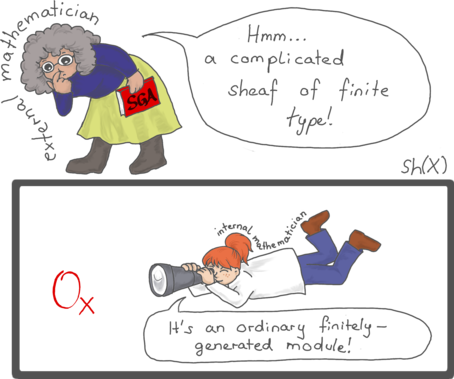
\includegraphics[scale=0.3]{images/external-internal-small}
  \medskip

  \hil{Anwendungen der internen Sprache von Topoi \\ in der algebraischen
  Geometrie}
  \medskip

  \scriptsize
  Ingo Blechschmidt
  \medskip

  Dissertationsprüfung am \\
  16. Oktober 2017
  \par
\end{frame}

% Orally: Laws of reasoning do not only apply to ordinary mathematical objects.
% They also apply to mathematical objects of different toposes. By cleverly
% choosing those topos, we can pretend that ...
% Any theorem automatically yields infinitely new theorems; sometimes, these
% are useful, and sometimes, they are indeed very nice.


\section[Interne Sprache]{Die interne Sprache von Topoi}

\subsection{Was ist ein Topos?}
\frame[t]{\frametitle{Was ist ein Topos?}
  \begin{block}{Formale Definition}Ein \hil{Topos} ist eine kartesisch
  abgeschlossene Kategorie, die alle endliche Limiten und einen
  Unterobjektklassifizierer besitzt.
  \end{block}

  \begin{block}{Motto}Ein Topos ist eine Kategorie, die hinreichend reich ist,
  um eine \hil{interne Sprache} zu erlauben.
  \end{block}

  \begin{block}{Beispiele}\begin{itemize}
    \item \hil{$\boldsymbol{\Set}$:} \tabto{1.5cm} die Kategorie der Mengen
    \item \hil{$\boldsymbol{\Sh(X)}$:} \tabto{1.5cm} die Kategorie der Garben auf einem Raum~$X$
    \item \hil{$\boldsymbol{\Zar(S)}$:} \tabto{1.5cm} der große Zariskitopos eines Basisschemas~$S$
  \end{itemize}\end{block}
}


\subsection{Was ist die interne Sprache?}

\frame[t]{\frametitle{Was ist die interne Sprache?}
  Die interne Sprache eines Topos~$\E$ erlaubt es, in einer \hil{naiven
  Element-basierten Sprache}
  \begin{enumerate}
    \item Objekte und Morphismen des Topos zu konstruieren,
    \item Aussagen über diese zu formulieren und
    \item solche Aussagen zu beweisen.
  \end{enumerate}

  \begin{center}
    \small
    \begin{tabular}{ll}
      \toprule
      extern & intern in $\E$ \\
      \midrule
      Objekt von~$\E$ & Menge \\
      Morphismus in~$\E$ & Abbildung zwischen Mengen \\
      Monomorphismus & injektive Abbildung \\
      Epimorphismus & surjektive Abbildung \\
      Gruppenobjekt & Gruppe \\
      \bottomrule
    \end{tabular}
  \end{center}
}
% Interne Sprache von Set nicht vergessen zu erwähnen!

\begin{frame}{Die interne Sprache von~$\boldsymbol{\Sh(X)}$}
  \small
  Sei~$X$ ein topologischer Raum. Dann definieren wir rekursiv
  \[ U \models \varphi \quad \text{("`$\varphi$ gilt auf~$U$"')} \]
  für offene Teilmengen~$U \subseteq X$ und Formeln~$\varphi$.
  \pause
  \[ \renewcommand{\arraystretch}{1.25}\begin{array}{@{}l@{\ }c@{\ }l@{}}
    U \models f = g \? \F &\Ll& f|_U = g|_U \in \F(U) \\
    U \models \varphi \wedge \psi &\Ll&
      \text{$U \models \varphi$ und $U \models \psi$} \\
    U \models \varphi \vee \psi &\Ll&
      \hcancel{\text{$U \models \varphi$ oder $U \models \psi$}}{0pt}{3pt}{0pt}{-2pt} \\
    && \text{es gibt eine Überdeckung $U = \bigcup_i U_i$ sd. für alle~$i$:} \\
    && \quad\quad \text{$U_i \models \varphi$ oder $U_i \models \psi$} \\
    U \models \varphi \Rightarrow \psi &\Ll&
      \text{für alle Offenen~$V \subseteq U$: } 
    \text{$V \models \varphi$ impliziert $V \models \psi$} \\
    U \models \forall f \? \F\_ \varphi(f) &\Ll&
      \text{für alle Schnitte~$f \in \F(V)$ auf~$V \subseteq U$: $V \models
      \varphi(f)$} \\
    U \models \exists f \? \F\_ \varphi(f) &\Ll&
      \text{es gibt eine Überdeckung~$U = \bigcup_i U_i$ sd. für alle~$i$} \\
    && \quad\quad \text{$f_i \in \F(U_i)$ mit
    $U_i \models \varphi(f_i)$ existiert}
  \end{array} \]
\end{frame}

\begin{frame}{Die interne Sprache von~$\boldsymbol{\Sh(X)}$}
  \begin{block}{Lokalität}
    Falls~$U = \bigcup_i U_i$, dann $U \models \varphi$ genau dann, falls $U_i
    \models \varphi$ für alle~$i$.
  \end{block}

  \begin{block}{Korrektheit}
    Falls~$U \models \varphi$ und falls $\varphi$
    \only<1>{konstruktiv}\only<2->{\pointthis{konstruktiv}{
      kein $\varphi \vee \neg\varphi$,\ \
      kein $\neg\neg\varphi \Rightarrow \varphi$,\ \
      kein Auswahlaxiom
    }} $\psi$ impliziert,
    dann~$U \models \psi$.
  \end{block}

  \vfill
  \vspace*{2em}

  \pause\pause
  \begin{block}{Ein erster Eindruck der konstruktiven Natur}
  \begin{itemize}
    \item $U \models f = 0$
      \tabto{2.9cm} genau dann, falls $f|_U = 0 \in \F(U)$.
    \item $U \models \neg\neg(f = 0)$
      \tabto{2.9cm} genau dann, falls~$f = 0$ auf einer dichten offenen
      Teilmenge von~$U$.
  \end{itemize}
  \end{block}
\end{frame}


\section[Kleiner Zariski]{Der kleine Zariskitopos eines Schemas}

\begin{frame}{Der kleine Zariskitopos}
  \begin{block}{Definition}Der \hil{kleine Zariskitopos} eines Schemas~$X$ ist
  die Kategorie~$\Sh(X)$ der mengenwertigen Garben auf~$X$.\end{block}
  \bigskip

  Aus interner Sicht von~$\Sh(X)$ \ldots
  \begin{itemize}
    \item \ \\[-1.2em]\mbox{sieht die Strukturgarbe~$\O_X$ wie ein \hil{gewöhnlicher Ring} und}
    \item \ \\[-1.2em]\mbox{eine Garbe von~$\O_X$-Moduln wie ein \hil{gewöhnlicher Modul}} über
    diesem Ring aus.
  \end{itemize}
\end{frame}

\backupstart
\begin{frame}[plain,c]
  \centering
  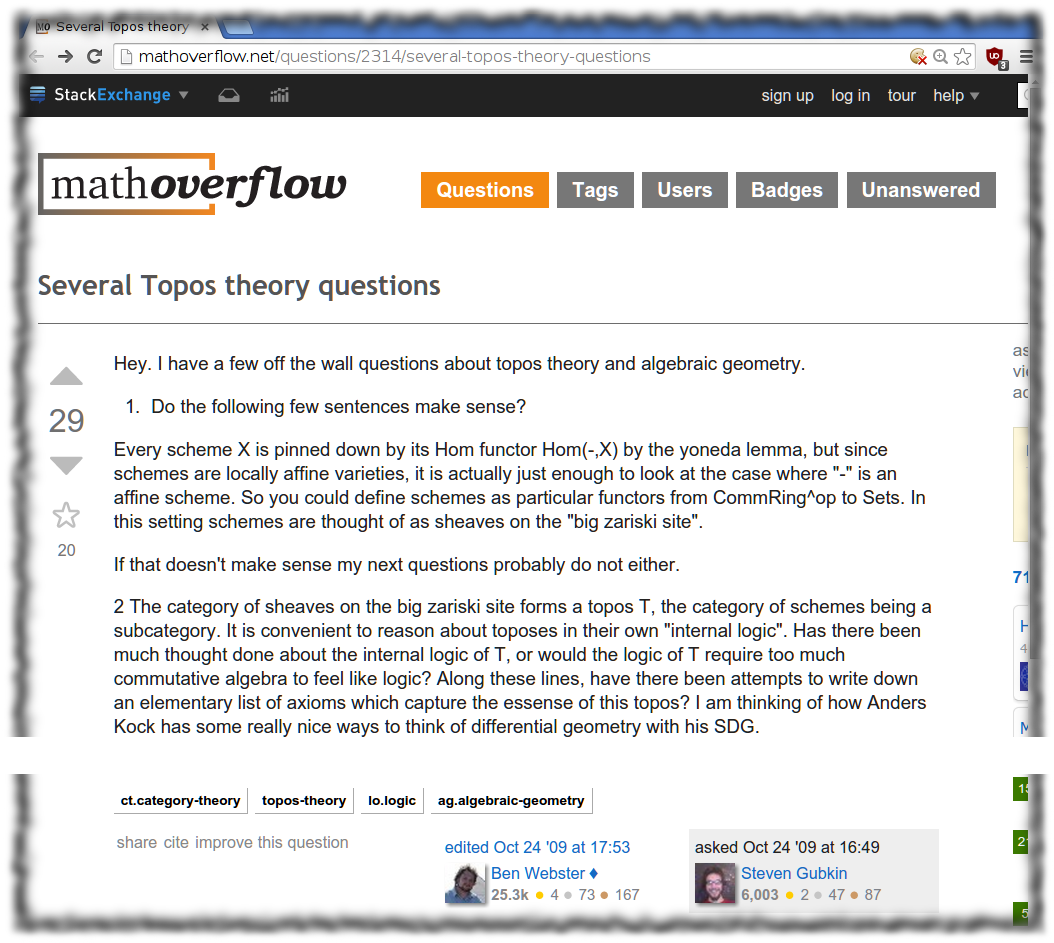
\includegraphics[scale=0.37]{images/math-overflow-steven-gubkin}
  \par
\end{frame}
\backupend


\subsection[Wörterbuch]{Entwicklung eines Wörterbuchs}

\begin{frame}{Entwicklung eines Wörterbuchs}
  \sloganwithoutborder{\hil{Verstehe Konzepte aus der algebraischen Geometrie
  als Konzepte aus der Algebra in der internen Welt von~$\boldsymbol{\Sh(X)}$.}}
  \begin{center}
    \small
    \scalebox{0.93}{\begin{tabular}{ll}
      \toprule
      extern & intern in $\Sh(X)$ \\
      \midrule
      Garbe von Mengen & Mengen \\
      Morphismus von Garben & Abbildung zwischen Mengen \\
      Monomorphismus & injektive Abbildung \\
      Epimorphismus & surjektive Abbildung \\
      \midrule
      Garbe von Ringen & Ring \\
      Garbe von Moduln & Modul \\
      Garbe von endlichem Typ & endlich erzeugter Modul \\
      lokal endlich freie Garbe & endlich freier Modul \\
      % coherent sheaf & coherent module \\
      Tensorprodukt von Garben & Tensorprodukt von Moduln \\
      Garbe der Differentialformen & Modul der Kählerdifferentiale \\
      % sheaf of rational functions & total quotient ring of~$\O_X$ \\
      Dimension von $X$ & Krulldimension von~$\O_X$ \\
      \bottomrule
    \end{tabular}}
  \end{center}

  \visible<2>{\begin{tikzpicture}[overlay]
    \draw[fill=white, draw=white, opacity=0.9] (0,0) rectangle (\paperwidth,6.6);
    \node[anchor=south west,inner sep=0] (image) at (1.8,1.3) {
      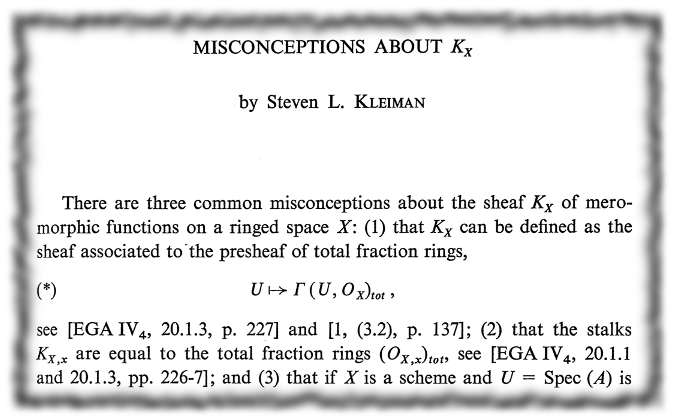
\includegraphics[width=0.7\textwidth]{images/steven-kleiman-misconceptions-about-kx}
    };
  \end{tikzpicture}}
\end{frame}

\begin{frame}{Anwendungen des Wörterbuchs}
  \vspace*{-2em}
  \begin{columns}[t]
    \begin{column}{0.51\textwidth}
      \begin{center}
        \begin{exampleblock}{}
          \justifying
          Sei~$0 \to M' \to M \to M'' \to 0$ eine kurze exakte Sequenz von
          Moduln. Sind~$M'$ und~$M''$ endlich erzeugt, so auch~$M$.
        \end{exampleblock}
        \medskip

        \scalebox{3}{$\Downarrow$}

        \begin{exampleblock}{}
          \justifying
          Sei $0 \to \F' \to \F \to \F'' \to 0$ eine kurze exakte Sequenz
          von~$\O_X$-Modulgarben. Sind~$\F'$ und~$\F''$ von endlichem Typ,
          so auch~$\F$.
        \end{exampleblock}
      \end{center}
    \end{column}
    \pause

    \begin{column}{0.39\textwidth}
      \begin{center}
        \begin{exampleblock}{}
          \justifying
          Jeder endlich erzeugte Vektorraum besitzt \emph{nicht nicht} eine
          Basis.
        \end{exampleblock}
        \medskip

        \scalebox{3}{$\Downarrow$}

        \begin{exampleblock}{}
          \justifying
          Jede Modulgarbe von endlichem Typ auf einem reduzierten Schema ist
          \emph{auf einer dichten offenen Teilmenge} lokal frei.
        \end{exampleblock}
        \centering
        \tiny Ravi Vakil: "`Important hard exercise"' (13.7.K).
        \par
      \end{center}
    \end{column}
  \end{columns}
\end{frame}

\begin{frame}{Mehr zum kleinen Zariskitopos}
  \vspace*{-2em}
  \slogan{\justifying Verstehe Konzepte und Sätze der \hil{algebraischen
  Geometrie} als Konzepte und Sätze der (konstruktiven) \hil{kommutativen
  Algebra} in der internen Welt des \hil{kleinen Zariskitopos}.}

%  In order to:
%  \begin{itemize}
%    \item Gain conceptual understanding.
%    \item Simplify proofs.
%    \item Develop a synthetic account of scheme theory.
%    \item Contribute to constructive algebra.
%  \end{itemize}

  \begin{itemize}
    \item Transferprinzipien~$M \leftrightarrow M^\sim$
    \item Besondere Eigenschaften der internen Welt
    \item Interne Charakterisierung von Quasikohärenz
    \item Logische Deutung von Ausbreitungsphänomenen
    \item Interne Konstruktion des relativen Spektrums
    \item Interner Beweis von Grothendiecks Lemma über generische Freiheit
  \end{itemize}
\end{frame}


\subsection{Transferprinzipien}

\begin{frame}\frametitle{Transferprinzipien}
  \begin{block}{Theorem}
    Die Strukturgarbe~$\O_{\Spec(A)}$ erbt all solche Eigenschaften erster
    Ordnung von~$A$, die stabil unter Lokalisierung sind.
  \end{block}

  \hil{Beweis.} Die Strukturgarbe~$\O_{\Spec(A)}$ ist die Lokalisierung
  \[ \underline{A}[\F^{-1}] \]
  \justifying
  der konstanten Garbe~$\underline{A}$ am \hil{generischen Filter}~$\F$,
  einer Garbe mit
  $\F_\ppp = A \setminus \ppp$.
  Die Ringe~$A$ und~$\underline{A}$ haben die gleichen Eigenschaften erster
  Ordnung.

  \hil{Bemerkung.} Die analoge Aussage gilt für~$A$-Moduln~$M$ und ihre Spiegelbilder~$M^\sim =
  \underline{M}[\F^{-1}]$.
\end{frame}


\subsection[Besonderheiten]{Besondere Eigenschaften der internen Welt}

\begin{frame}{Besonderheiten der internen Welt}
  Sei~$X$ ein Schema. Intern in~$\Sh(X)$ gilt:
  \begin{center}
    \hil{Jedes nicht-invertierbare Element \\ von~$\boldsymbol{\O_X}$ ist nilpotent.}
  \end{center}

  \only<1>{
    \centering
    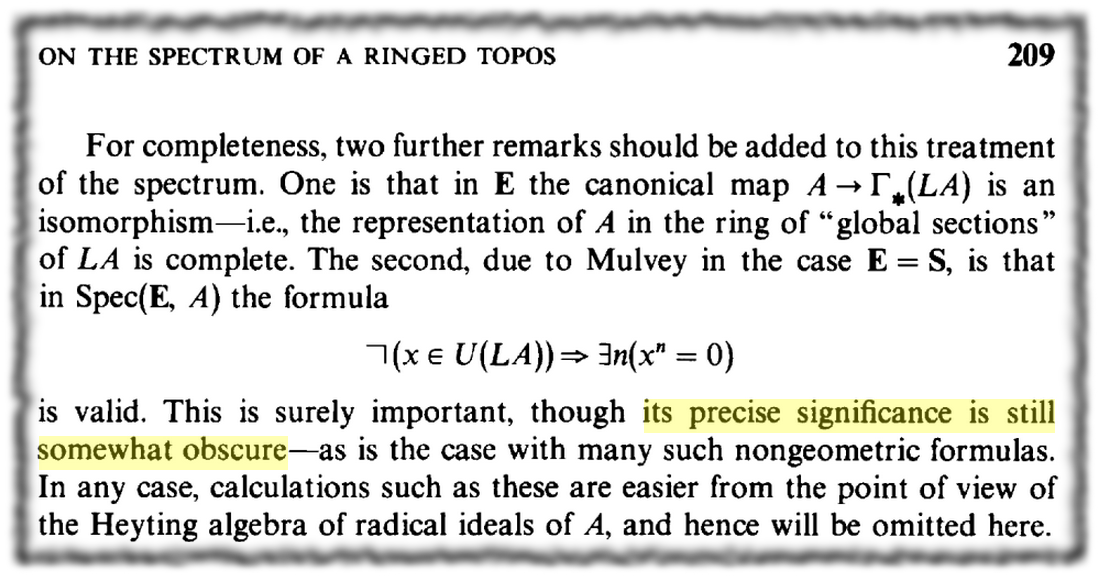
\includegraphics[scale=0.25]{images/tierney-on-the-spectrum-of-a-ringed-topos} \\
    \tiny
    %Miles Tierney. ``On the spectrum of a ringed topos''. \\ In: \emph{Algebra,
    %Topology, and Category Theory. A Collection of Papers in Honor of Samuel
    %Eilenberg}. Ed.\@ by A.~Heller and M.~Tierney. Academic Press, 1976,
    %pp.~189--210.
    Miles Tierney. On the spectrum of a ringed topos. 1976.
    \par
  }

  \only<2>{
    Ist~$X$ reduziert, so folgt daraus für die interne Welt:
    \begin{itemize}
      \item $\O_X$ ist ein \hil{Körper}: Nichteinheiten sind Null.
      \item $\O_X$ hat \hil{$\boldsymbol{\neg\neg}$-stabile Gleichheit}: $\neg\neg(x = 0)
      \Rightarrow x = 0$.
      \item $\O_X$ is \hil{anonym noethersch}: Jedes Ideal von~$\O_X$ ist
      \mbox{\hil{nicht nicht}} endlich erzeugt.
    \end{itemize}
  }
\end{frame}


\subsection[Gen. Freiheit]{Grothendiecks Lemma über generische Freiheit}

\begin{frame}{Generische Freiheit}
  Sei~$A$ ein reduzierter Ring und seien~$B, M$ wie folgt:

  \vspace*{-4.75em}
  ${\qquad\qquad\qquad\quad\qquad\qquad\qquad\qquad\qquad\qquad\qquad}\xymatrixcolsep{3.5pc}\xymatrixrowsep{2pc}\xymatrix{
    & \ar@{-}[d]_{\substack{\text{endlich}\\\text{erzeugt}}} M \\
    A \ar[r]_{\text{veT}} & B
  }$

  \hil{Theorem.} Ist~$1 \neq 0$ in~$A$, so gibt es $f \neq 0$ in $A$ sodass
  \begin{enumerate}
    \item $B[f^{-1}]$ und $M[f^{-1}]$ als Moduln über $A[f^{-1}]$ frei sind,
    \item $A[f^{-1}] \to B[f^{-1}]$ von endlicher Präsentation ist und
    \item $M[f^{-1}]$ als Modul über~$B[f^{-1}]$ endlich präsentiert ist.
  \end{enumerate}
  \pause

  \hil{Konstruktive Version.} Ist Null das einzige Element~$f \in A$ mit
  {\renewcommand{\insertenumlabel}{1}\usebeamertemplate{enumerate item}},
  {\renewcommand{\insertenumlabel}{2}\usebeamertemplate{enumerate item}} und
  {\renewcommand{\insertenumlabel}{3}\usebeamertemplate{enumerate item}},
  so~$1 = 0 \in A$.
  \pause

  \hil{Beweis.} Die Behauptung ist die Übersetzung des trivialen Fakts, dass
  intern in~$\Sh(\Spec(A))$ es \hil{nicht nicht} der Fall ist, dass
  \begin{enumerate}
    \item $B^\sim$ und~$M^\sim$ als Moduln über~$A^\sim$ frei sind,
    \item $A^\sim \to B^\sim$ von endlicher Präsentation ist und
    \item $M^\sim$ als Modul über~$B^\sim$ endlich präsentiert ist.
  \end{enumerate}
\end{frame}

\begin{frame}
  \small\justifying
  Sei~$B^\sim$ als~$A^\sim$-Modul von~$(x^i y^j)_{i,j\geq0}$ erzeugt.
  Es ist \hil{nicht nicht} der Fall, dass entweder ein Erzeuger als
  Linearkombination von Erzeugern mit kleinerem Index ausgedrückt werden kann,
  oder nicht.\par

  \centering
  \begin{tikzpicture}[scale=0.4]
    \begin{scope}
      \draw[step=1cm,gray,very thin] (0,0) grid (8,8);

      \draw
        (0,8) -- (0,0) -- (8,0);

      \fill[fill=blue!40!white,opacity=0.5]
        (0,8) -- (0,0) -- (6,0) -- (6,5) -- (5,5) -- (5,8);

      \fill[fill=red!40!white,opacity=0.5]
        (5,5) -- (6,5) -- (6,6) -- (5,6);

      \node[shape=circle,draw,inner sep=2pt] at (1,1) {1};
    \end{scope}

    \begin{scope}[xshift=9cm]
      \draw[step=1cm,gray,very thin] (0,0) grid (8,8);

      \draw
        (0,8) -- (0,0) -- (8,0);

      \fill[pattern=north east lines,pattern color=gray,opacity=0.5]
        (5,8) -- (5,5) -- (8,5) -- (8,8);
      \draw
        (5,8) -- (5,5) -- (8,5);

      \fill[fill=blue!40!white,opacity=0.5]
        (0,8) -- (0,0) -- (3,0) -- (3,5) -- (2,5) -- (2,8);

      \fill[fill=red!40!white,opacity=0.5]
        (2,5) -- (3,5) -- (3,6) -- (2,6);

      \node[shape=circle,draw,inner sep=2pt] at (1,1) {2};
    \end{scope}

    \begin{scope}[xshift=18cm]
      \draw[step=1cm,gray,very thin] (0,0) grid (8,8);

      \draw
        (0,8) -- (0,0) -- (8,0);

      \fill[pattern=north east lines,pattern color=gray,opacity=0.5]
        (2,8) -- (2,5) -- (8,5) -- (8,8);
      \draw
        (2,8) -- (2,5) -- (8,5);

      \fill[fill=blue!40!white,opacity=0.5]
        (0,8) -- (0,0) -- (7,0) -- (7,2) -- (6,2) -- (6,5) -- (2,5) -- (2,8);

      \fill[fill=red!40!white,opacity=0.5]
        (6,2) -- (7,2) -- (7,3) -- (6,3);

      \node[shape=circle,draw,inner sep=2pt] at (1,1) {3};
    \end{scope}

    \begin{scope}[yshift=-9cm]
      \draw[step=1cm,gray,very thin] (0,0) grid (8,8);

      \draw
        (0,8) -- (0,0) -- (8,0);

      \fill[pattern=north east lines,pattern color=gray,opacity=0.5]
        (2,8) -- (2,5) -- (6,5) -- (6,2) -- (8,2) -- (8,8);
      \draw
        (2,8) -- (2,5) -- (6,5) -- (6,2) -- (8,2);

      \fill[fill=blue!40!white,opacity=0.5]
        (0,8) -- (0,0) -- (6,0) -- (6,3) -- (5,3) -- (5,5) -- (2,5) -- (2,8);

      \fill[fill=red!40!white,opacity=0.5]
        (5,3) -- (6,3) -- (6,4) -- (5,4);

      \node[shape=circle,draw,inner sep=2pt] at (1,1) {4};
    \end{scope}

    \begin{scope}[yshift=-9cm,xshift=9cm]
      \draw[step=1cm,gray,very thin] (0,0) grid (8,8);

      \draw
        (2,8) -- (2,5) -- (5,5) -- (5,3) -- (6,3) -- (6,2) -- (8,2);

      \draw
        (0,8) -- (0,0) -- (8,0);

      \fill[pattern=north east lines,pattern color=gray,opacity=0.5]
        (2,8) -- (2,5) -- (5,5) -- (5,3) -- (6,3) -- (6,2) -- (8,2) -- (8,8);

      \fill[fill=blue!40!white,opacity=0.5]
        (0,8) -- (0,0) -- (4,0) -- (4,3) -- (3,3) -- (3,5) -- (2,5) -- (2,8);

      \fill[fill=red!40!white,opacity=0.5]
        (3,3) -- (4,3) -- (4,4) -- (3,4);

      \node[shape=circle,draw,inner sep=2pt] at (1,1) {5};
    \end{scope}

    \begin{scope}[yshift=-9cm,xshift=18cm]
      \draw[step=1cm,gray,very thin] (0,0) grid (8,8);

      \draw
        (0,8) -- (0,0) -- (8,0);

      \fill[pattern=north east lines,pattern color=gray,opacity=0.5]
        (2,8) -- (2,5) -- (3,5) -- (3,3) -- (6,3) -- (6,2) -- (8,2) -- (8,8);
      \draw
        (2,8) -- (2,5) -- (3,5) -- (3,3) -- (6,3) -- (6,2) -- (8,2);

      \node[shape=circle,draw,inner sep=2pt] at (1,1) {6};
    \end{scope}
  \end{tikzpicture}
  \par
\end{frame}

\section[Großer Zariski]{Der große Zariskitopos eines Schemas}

\begin{frame}{Synthetische algebraische Geometrie}
  Üblicher Zugang zur Schematheorie: \hil{Entwickle Schematheorie über
  gewöhnlicher Mengenlehre} mit
  \begin{itemize}
    \item lokal geringten Räumen oder
    \small
    \begin{multline*}
      \text{Menge der Primideale von~$\ZZ[X,Y,Z]/(X^n+Y^n-Z^n)$} + {} \\
      \text{Zariskitopologie} + \text{Strukturgarbe}
    \end{multline*}
    \normalsize
    \item Grothendiecks Punktefunktoransatz, bei dem ein Schema ein
    Funktor~$\mathrm{Ring} \to \mathrm{Set}$ ist.
    \small\[ A \longmapsto \{ (x,y,z) \? A^3 \,|\, x^n+y^n-z^n=0 \} \]
  \end{itemize}
  \bigskip
  \pause

  \hil{Synthetischer Zugang:} Modelliere Schemata \hil{direkt als Mengen} in
  einer nichtklassischen Mengentheorie.
  \small
  \[ \{ (x,y,z) \? (\affl)^3 \,|\, x^n+y^n-z^n=0 \} \]
\end{frame}

\begin{frame}{Der große Zariskitopos}
  \begin{block}{Definition}\justifying
  Der \hil{große Zariskitopos} $\Zar(S)$ eines
  Schemas~$S$ ist die Kategorie $\Sh(\Aff/S)$ derjenigen Funktoren
  $(\Aff/S)^\op \to \Set$, die die Verklebebedingung erfüllen: Für jedes
  affine Schema~$U = \bigcup_i U_i$ über~$S$ soll
  \[ F(U) \to
    \prod_i F(U_i) \rightrightarrows
    \prod_{j,k} F(U_j \cap U_k) \]
  \\[-0.6em]
  ein Limesdiagramm sein.
  \end{block}

  \begin{itemize}
    \item Der Punktefunktor~$\ull{X} =
    \Hom_S(\cdot,X)$ eines~$S$-Schemas~$X$ ist ein Objekt von~$\Zar(S)$.
    "`Die \hil{Menge der Punkte} von~$X$."'
    \item In der internen Welt ist $\affl$
    ein Körper:
    \[ \Zar(S) \models \forall x\?\affl\_ x \neq 0 \Longrightarrow \text{$x$ invertierbar} \]
  \end{itemize}
\end{frame}


\subsection{Synthetische Konstruktionen}

\begin{frame}{Synthetische Konstruktionen}
  \begin{itemize}
  \item $\mathbb{P}^n = \{ (x_0,\ldots,x_n) : (\affl)^{n+1} \,|\,
    x_0 \neq 0 \vee \cdots \vee x_n \neq 0 \}/(\affl)^\times$ \\
  $\phantom{\mathbb{P}^n} \cong \text{Menge der eindimensionalen UVR von~$(\affl)^{n+1}$}$.

  \begin{itemize}
    \item $\O(1) = (\ell^\vee)_{\ell : \mathbb{P}^n}$
    \item $\O(-1) = (\ell)_{\ell : \mathbb{P}^n}$
    \item Eulersequenz: $0 \to \ell^\perp \to ((\affl)^{n+1})^\vee \to \ell^\vee \to 0$
  \end{itemize}\bigskip

  \item $\RelSpec R = \Hom_{\mathrm{Alg}(\affl)}(R, \affl)$ \\
  $\phantom{\RelSpec R} = \text{Menge der $\affl$-wertigen Punkte von $R$}.$

  \begin{itemize}
    \item $\RelSpec \affl[X,Y,Z]/(X^n+Y^n-Z^n) \cong {}$ \\ \qquad\qquad $\{ (x,y,z) \? (\affl)^3 \,|\, x^n+y^n-z^n = 0 \}$ \medskip
    \item $\Delta \defeq \RelSpec \affl[\varepsilon]/(\varepsilon^2) \cong \{ \varepsilon : \affl \,|\, \varepsilon^2 = 0 \}$
  \end{itemize}\bigskip

  \item $TX = \Hom(\Delta, X)$.
  \end{itemize}
\end{frame}


\subsection{Synthetische Eigenschaften}

\begin{frame}{Formulierung von Eigenschaften}
  \begin{block}{Definition}
    \small
    Ein~$\affl$-Modul~$E$ ist genau dann \hil{synthetisch quasikohärent}, wenn
    \vspace*{-0.5em}
    \[ E \otimes_\affl R \longrightarrow E^{\Spec R} \]
    \vspace*{-1.7em}

    für alle endlich präsentierten~$\affl$-Algebren~$R$ ein Isomorphismus ist.
    (Dabei $\Spec R = \Hom_{\mathrm{Alg}(\affl)}(R, \affl)$.)
  \end{block}

  \begin{itemize}
  \item Aus der synthetischen Quasikohärenz von~$\affl$ folgt:

  Jede Abbildung $\affl \to \affl$ ist polynomiell.

  \item\justifying Offene und abgeschlossene Immersionen, quasikompakte und
  quasiseparierte Morphismen, synthetische Schemata, eigentliche Morphismen,
  \ldots

  \item Charakterisierung von wichtigen Untertopoi wie dem \hil{étalen Topos}
  oder dem \hil{fppf-Topos}
  \end{itemize}
\end{frame}


\backupstart

\section{Offene Fragen}

\begin{frame}{Offene Fragen}
  \begin{itemize}
    \small
    \item Wie geht Kohomologie in der internen Welt wirklich?
    \item Welche Theorien klassifizieren relevante Untertopoi?
    \item Welche Anwendungen liefern andere Topologien?
    \item Was ist der Bezug zu den dynamischen Methoden der Algebra?
    \item Wie sollte synthetische algebraische Geometrie weiter entwickelt
    werden?
  \end{itemize}

  {\vspace{-0.1em}\centering
  \rotatebox{90}{\tiny\scalebox{0.5}{Illustration: Carina Willbold}}\hspace{-0.05cm}%
  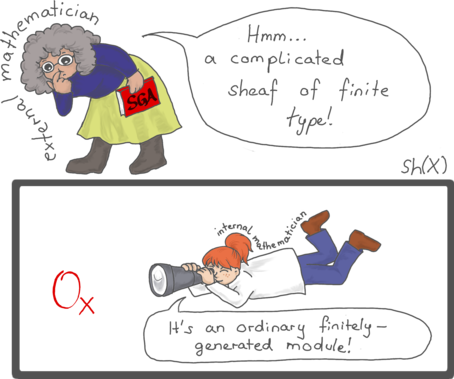
\includegraphics[scale=0.28]{images/external-internal-small}
  \par\medskip\vspace{-0.1em}}
\end{frame}

\backupend

\backupstart


\appendix


\section{Spreading from points to neighbourhoods}

\begin{frame}\frametitle{Spreading from points to neighbourhoods}
  All of the following lemmas have a short, sometimes trivial proof.
  Let~$\F$ be a sheaf of finite type on a ringed space~$X$.
  Let~$x \in X$. Let~$A \subseteq X$ be a closed subset. Then:
  \small
  \begin{enumerate}
    \item $\F_x = 0$ iff~$\F|_U = 0$ for some open neighbourhood of~$x$.
    \item $\F|_A = 0$ iff~$\F|_U = 0$ for some open set containing~$A$.
    \item $\F_x$ can be generated by~$n$ elements iff this is true on some open
    neighbourhood of~$x$.
%   \item $\alpha_x$ is surjective iff~$\alpha$ is an epimorphism on some open
%   set containing~$x$, where~$\alpha : \G \to \F$ is any morphism.
    \item $\mathcal{H}\mathrm{om}_{\O_X}(\F,\G)_x \cong
    \Hom_{\O_{X,x}}(\F_x,\G_x)$ if~$\F$ is of finite presentation around~$x$.
    \item $\F$ is torsion iff~$\F_\xi$ vanishes (assume~$X$ integral and~$\F$ quasicoherent).
    \item $\F$ is torsion iff~$\F|_{\mathrm{Ass}(\O_X)}$ vanishes (assume~$X$
    locally Noetherian and~$\F$ quasicoherent).
  \end{enumerate}
\end{frame}


\subsection{Quasicoherence}

\begin{frame}\frametitle{Quasicoherence}
  Let~$X$ be a scheme. Let~$\E$ be an~$\O_X$-module.

  Then~$\E$ is quasicoherent
  if and only if, internally to~$\Sh(X)$,
  \begin{quote}\textnormal{$\E[f^{-1}]$ is a $\Box_f$-sheaf for any~$f : \O_X$, \\[0.3em]
  \qquad\qquad where~$\Box_f\varphi \defeqv (\text{$f$ invertible} \Rightarrow \varphi)$.}
  \end{quote}
  \pause

  In particular: If~$\E$ is quasicoherent, then internally
  \[ (\text{$f$ invertible} \Rightarrow s = 0) \Longrightarrow
    \bigvee_{n \geq 0} f^n s = 0 \]
  \vspace*{-1.5em}\par%
  for any~$f : \O_X$ and~$s : \E$.
\end{frame}

\note{\justifying
  The sheaf condition and the sheafification functor can be described purely
  internally. An object~$M$ is \emph{separated} with respect to~$\Box$ if
  and only if, from the internal point of view,
  \[ \forall x,y : M\_\ \Box(x = y) \Rightarrow x = y. \]
  It is a \emph{sheaf} with respect to~$\Box$, if furthermore
  \[ \forall K \subseteq M\_\
    \Box(\exists x : M\_\ K = \{ x \}) \Longrightarrow
    \exists x : M\_\ \Box(x \in K). \]

  The second condition displayed on the previous slide is equivalent to the
  separatedness condition. In the special case~$\E = \O_X$, $s = 1$ it reduces
  to Mulvey's ``somewhat obscure formula''. We now understand this condition in
  its proper context.
  \par
}


\subsection[Spreading]{Spreading of properties}

\newcommand{\idiamond}{{\usebeamercolor[fg]{item}{\boldsymbol{\Box}}}}
\newcommand{\gdiamond}[1]{\textcolor{gray}{\boldsymbol{\Box}(}#1\textcolor{gray}{)}}

\begin{frame}\frametitle{The $\Box$-translation}
  Let~$\E_\Box \hookrightarrow \E$ be a subtopos given by a local
  operator. Then
  \[ \E_\Box \models \varphi \qquad\text{iff}\qquad
    \E \models \varphi^\Box\only<2->{.}\only<1>{,}\]
  \only<1>{where the translation~$\varphi \mapsto \varphi^\Box$ is given by:
  \begin{align*}
    (s = t)^\Box &\defeqv \idiamond(s=t) \\
    (\varphi \wedge \psi)^\Box &\defeqv \gdiamond{\varphi^\Box \wedge \psi^\Box} \\
    (\varphi \vee \psi)^\Box &\defeqv \idiamond(\varphi^\Box \vee \psi^\Box) \\
    (\varphi \Rightarrow \psi)^\Box &\defeqv \gdiamond{\varphi^\Box \Rightarrow \psi^\Box} \\
    (\forall x\?X\_ \varphi(x))^\Box &\defeqv \gdiamond{\forall x\?X\_ \varphi^\Box(x)} \\
    (\exists x\?X\_ \varphi(x))^\Box &\defeqv \idiamond(\exists x\?X\_ \varphi^\Box(x))
  \end{align*}}%
  \only<2->{%
    Let~$X$ be a scheme. Depending on~$\Box$,~$\Sh(X)
    \models \Box\varphi$ means that~$\varphi$ holds on \ldots
    \begin{itemize}
      \item \ldots{} a dense open subset.
      \item \ldots{} a schematically dense open subset.
      \item \ldots{} a given open subset~$U$.
      \item \ldots{} an open subset containing a given closed subset~$A$.
      \item \ldots{} an open neighbourhood of a given point~$x \in X$.
    \end{itemize}

    \pause
    Can tackle the question~``$\varphi^\Box \stackrel{?}{\Rightarrow} \Box\varphi$'' logically.
  }
\end{frame}

\note{\justifying
  The~$\Box$-translation is a generalization of the \emph{double negation
  translation}, which is well-known in logic. The double negation translation
  has the following curious property: A formula~$\varphi$ admits a classical
  proof if and only if the translated formula~$\varphi^{\neg\neg}$ admits an
  intuitionistic proof.

  The~$\Box$-translation has been studied before (see for instance Aczel:
  \emph{The Russell--Prawitz modality}, and Escardó, Oliva: \emph{The Peirce
  translation and the double negation shift}), but to the best of my know\-ledge,
  this application -- expressing the internal language of
  subtoposes in the internal language of the ambient topos -- is new.
  \par
}

\note{\justifying
  For ease of exposition, assume that~$X$ is irreducible with generic
  point~$\xi$. Let~$\Box \defeqv \neg\neg$.

  Then~$\Sh(X) \models \Box \varphi$ means that~$\varphi$ holds on a dense
  open subset of~$X$, while~$\Sh(X) \models \varphi^\Box$ means
  that~$\varphi$ holds at the generic point (taking stalks of all involved
  sheaves).

  The question~``does~$\varphi^\Box$ imply~$\Box\varphi$?'' therefore
  means: Does~$\varphi$ spread from the generic point to a dense open subset?

  For the special case of the double negation translation, a general answer to
  this purely logical question has long been known: This holds if~$\varphi$ is
  a \emph{geometric formula} (doesn't contain~$\Rightarrow$ and~$\forall$).
  \par
}

\note{\justifying
  Let~$\F$ be a sheaf of modules on a locally ringed space~$X$.
  Assume that the stalk~$\F_x$ at some point~$x \in X$ vanishes.
  Then in general it does \emph{not} follow that~$\F$ vanishes on some open
  neighbourhood of~$x$.

  This can be understood in logical terms: The statement that~$\F$ vanishes,
  \[ \forall s : \F\_\ s = 0, \]
  is not a geometric formula.

  However, if~$\F$ is additionally supposed to be of finite type, then it
  \emph{does} follow that~$\F$ vanishes on an open neighbourhood. This too can
  be understood in logical terms: If~$\F$ is of finite type, then internally
  there are generators~$s_1,\ldots,s_n$ of~$\F$. Thus the vanishing of~$\F$ can
  be reformulated as
  \[ s_1 = 0 \wedge \cdots \wedge s_n = 0, \]
  and this condition is manifestly geometric.
  \par
}


\subsection[Relative spectrum]{The relative spectrum}

\newcommand{\defspeca}{\text{topological space of the prime ideals of $A$}}
\newcommand{\defspecb}{\text{topological space of the prime filters of $A$}}
\newcommand{\defspecc}{\text{locale of the prime filters of $A$}}

\begin{frame}\frametitle{The absolute spectrum, internalised}
  Let~$A$ be a commutative ring in a topos~$\E$.

  To construct the \hil{free local ring} over~$A$, give a constructive account
  of the spectrum:
  \begin{align*}
    \only<1>{\Spec A &\defeq \defspeca}
    \only<2->{\Spec A &\defeq \hcancel{$\defspeca$}{0pt}{3pt}{0pt}{-2pt}}
    \\
    \only<3>{&\defeq \defspecb}
    \only<4->{&\defeq \hcancel{$\defspecb$}{0pt}{3pt}{0pt}{-2pt}}
    \\
    \only<5->{&\defeq \defspecc}
  \end{align*}
  \pause
  \pause
  \pause
  \pause
  The frame of opens of~$\Spec A$ is the frame of radical ideals
  in~$A$. Universal property:
  \[ \Hom_{\mathrm{LRT}/|\E|}(T, \Spec A) \cong \Hom_{\mathrm{Ring}(\E)}(A, \mu_*\O_T) \]
  for all locally ringed toposes~$T$ equipped with a geometric morphism~$T \xrightarrow{\mu} \E$.
\end{frame}

\note{\justifying
  The axioms of a prime filter constitute a propositional geometric theory.
  Therefore there exists the \emph{classifying locale} over prime filters. This
  is the ring's spectrum. See Vicker's
  \href{http://www.cs.bham.ac.uk/~sjv/LocTopSpaces.pdf}{Locales and Toposes as Spaces} and
  \href{http://www.cs.bham.ac.uk/~sjv/GeoAspects.pdf}{Continuity and geometric
  logic} for very accessible introductions to this topic.

  Monique Hakim constructed in her thesis a very general spectrum functor,
  taking a ringed topos to a locally ringed one, using explicit calculations
  with sites.

  Using the internal language allows to reduce these calculations to a minimum.
  One constructs the spectrum as the sheaf topos over an internal
  locale and then uses the general theorem that toposes over the base~$\E$ are
  the same as toposes internal to~$\E$.

  As a byproduct one obtains that Hakim's spectrum is \emph{localic} over the base.
  \par
}

\begin{frame}\frametitle{The relative spectrum}
  Let~$X$ be a scheme and~$\A$ be a quasicoherent~$\O_X$-algebra.
  Can we describe its \hil{relative spectrum}~$\RelSpec_X \A \to X$ internally?

  Desired universal property:
  \[ \Hom_{\mathrm{LRL}/X}(T, \RelSpec_X \A) \cong \Hom_{\mathrm{Alg}(\O_X)}(\A,
  \mu_*\O_T) \]
  for all locally ringed locales~$T$ over~$X$.
  \pause

  \only<2>{\begin{exampleblock}{Beware of believing false statements}
  \begin{itemize}
  \item $\RelSpec_X \O_X = X$.
  \item $\Spec \A$ is the one-point locale iff every element
  of~$\A$ is invertible or nilpotent.
  \item Every element of~$\O_X$ which is not invertible is nilpotent.
  \item Thus cannot prove~$\Spec \O_X = \mathrm{pt}$ internally.
  \end{itemize}\end{exampleblock}}
  \pause

  \hil{Solution:} Define internally the frame of~$\RelSpec_X \A$ to be the frame of
  those radical ideals~$I \subseteq \A$ such that
  \[ \forall f\?\O_X\_ \forall s\?\A\_
    (\text{$f$ invertible in~$\O_X$} \Rightarrow s \in I) \Longrightarrow
      fs \in I. \]
  \pause
  Its \hil{points} are those prime filters~$G$ of~$\A$ such that
  \[ \forall f\?\O_X\_ \varphi(f) \in G \Longrightarrow \text{$f$ invertible in~$\O_X$}. \]
\end{frame}

\note{\justifying
  The stated condition on~$I$ is, under the assumption that~$\A$ is
  quasicoherent, equivalent to the condition that~$I$ is quasicoherent (as
  an~$\O_X$-module).

  The relative spectrum is thus constructed as a certain sublocale of the
  absolute one. The two constructions coincide if and only if the dimension of
  the base scheme is~$\leq 0$.

  If~$X$ is not a scheme or~$\A$ is not quasicoherent, the construction still
  gives rise to a locally ringed locale over~$X$ which satisfies the universal
  property
  \[ \Hom_{\mathrm{LRL}/X}(T, \RelSpec_X \A) \cong \Hom_{\mathrm{Alg}(\O_X)}(\A,
  \mu_*\O_T) \]
  for all locally ringed locales~$T \xrightarrow{\mu} X$ over~$X$.
  \par
}

\begin{frame}\frametitle{The relative spectrum, reformulated}
  Let~$B \to A$ be an algebra in a topos.

  Is there a \hil{free local and local-over-$\boldsymbol{B}$ ring}~$A \to A'$ over~$A$?

  \[ \xymatrix{
    B \ar[r]\ar@/^2pc/[rrrr]^{\text{local}}\ar@/_/[rrd]_[@!-33]{\text{local}} &
      A \ar[rd] \ar[rrr] &&&
      {\substack{\text{local}\\\text{\normalsize$R$}\\\phantom{\text{local}}}} \\
    && {\substack{\text{\normalsize$A'$}\\\text{local}}} \ar@{-->}[rru]_[@!35]{\text{local}}
  } \]

  \medskip
  Form limits in the category of \hil{locally ringed locales}
  by \hil{relocalising} the corresponding limit in ringed locales.
\end{frame}

\note{\justifying
  One might wonder whether the absolute spectrum or the relative one is ``more
  fundamental''. The absolute spectrum can be expressed using the relative one,
  since
  \[ \Spec A = \RelSpec_{\Spec \ZZ} A^{\sim}, \]
  but the other way is not in general possible: The absolute spectrum is always
  (quasi-)compact, while the relative one is not in general.
  \par
}
% XXX: Give details.


\subsection{The étale subtopos}

\begin{frame}\frametitle{The étale subtopos}
  Recall that the \hil{Kummer sequence} is not exact in~$\Zar(S)$ at the third
  term:
  \[ 1 \lra \mu_n \lra (\affl)^\times \stackrel{(\cdot)^n}{\lra} (\affl)^\times \lra 1 \]
  But we have:
  \[ \Zar(S) \models \forall f\?(\affl)^\times\_ \Box_\text{ét}(\exists
  g\?(\affl)^\times\_ f = g^n), \]
  where~$\Box_\text{ét}$ is such that $\Zar(S)_{\Box_\text{ét}}
  \hookrightarrow \Zar(S)$ is the \hil{big étale topos} of~$S$. It is the largest
  subtopos of~$\Zar(S)$ where
  \[ \speak{$\affl$ is separably closed} \]
  holds [reinterpretation of Wraith, PSSL~1].
\end{frame}

\backupend

\end{document}
